% Created 2024-11-12 Tue 03:52
% Intended LaTeX compiler: pdflatex
\documentclass[11pt]{article}
\usepackage[utf8]{inputenc}
\usepackage[T1]{fontenc}
\usepackage{graphicx}
\usepackage{longtable}
\usepackage{wrapfig}
\usepackage{rotating}
\usepackage[normalem]{ulem}
\usepackage{amsmath}
\usepackage{amssymb}
\usepackage{capt-of}
\usepackage{hyperref}
\usepackage[polish]{babel}
\usepackage[T1]{fontenc}
\usepackage[utf8]{inputenc}
\selectlanguage{polish}
\usepackage{caption}
\usepackage{booktabs}
\captionsetup{labelfont=bf}
\usepackage{float}
\usepackage[a4paper, total={6in, 8in}]{geometry}
\author{Piotr Karamon}
\date{12.11.2024r.}
\title{Laboratorium 5 - Problem pięciu filozofów}
\hypersetup{
 pdfauthor={Piotr Karamon},
 pdftitle={Laboratorium 5 - Problem pięciu filozofów},
 pdfkeywords={},
 pdfsubject={},
 pdfcreator={Emacs 29.2 (Org mode 9.7.11)}, 
 pdflang={Polish}}

% Setup for code blocks [1/2]

\usepackage{fvextra}

\fvset{%
  commandchars=\\\{\},
  highlightcolor=white!95!black!80!blue,
  breaklines=true,
  breaksymbol=\color{white!60!black}\tiny\ensuremath{\hookrightarrow}}

% Make line numbers smaller and grey.
\renewcommand\theFancyVerbLine{\footnotesize\color{black!40!white}\arabic{FancyVerbLine}}

\usepackage{xcolor}

% In case engrave-faces-latex-gen-preamble has not been run.
\providecolor{EfD}{HTML}{f7f7f7}
\providecolor{EFD}{HTML}{28292e}

% Define a Code environment to prettily wrap the fontified code.
\usepackage[breakable,xparse]{tcolorbox}
\DeclareTColorBox[]{Code}{o}%
{colback=EfD!98!EFD, colframe=EfD!95!EFD,
  fontupper=\footnotesize\setlength{\fboxsep}{0pt},
  colupper=EFD,
  IfNoValueTF={#1}%
  {boxsep=2pt, arc=2.5pt, outer arc=2.5pt,
    boxrule=0.5pt, left=2pt}%
  {boxsep=2.5pt, arc=0pt, outer arc=0pt,
    boxrule=0pt, leftrule=1.5pt, left=0.5pt},
  right=2pt, top=1pt, bottom=0.5pt,
  breakable}

% Support listings with captions
\usepackage{float}
\floatstyle{plain}
\newfloat{listing}{htbp}{lst}
\newcommand{\listingsname}{Listing}
\floatname{listing}{\listingsname}
\newcommand{\listoflistingsname}{List of Listings}
\providecommand{\listoflistings}{\listof{listing}{\listoflistingsname}}


% Setup for code blocks [2/2]: syntax highlighting colors

\newcommand\efstrut{\vrule height 2.1ex depth 0.8ex width 0pt}
\definecolor{EFD}{HTML}{000000}
\definecolor{EfD}{HTML}{ffffff}
\newcommand{\EFD}[1]{\textcolor{EFD}{#1}} % default
\definecolor{EFvp}{HTML}{000000}
\newcommand{\EFvp}[1]{\textcolor{EFvp}{#1}} % variable-pitch
\definecolor{EFh}{HTML}{7f7f7f}
\newcommand{\EFh}[1]{\textcolor{EFh}{#1}} % shadow
\definecolor{EFsc}{HTML}{228b22}
\newcommand{\EFsc}[1]{\textcolor{EFsc}{\textbf{#1}}} % success
\definecolor{EFw}{HTML}{ff8e00}
\newcommand{\EFw}[1]{\textcolor{EFw}{\textbf{#1}}} % warning
\definecolor{EFe}{HTML}{ff0000}
\newcommand{\EFe}[1]{\textcolor{EFe}{\textbf{#1}}} % error
\definecolor{EFl}{HTML}{ff0000}
\newcommand{\EFl}[1]{\textcolor{EFl}{#1}} % link
\definecolor{EFlv}{HTML}{ff0000}
\newcommand{\EFlv}[1]{\textcolor{EFlv}{#1}} % link-visited
\definecolor{EFhi}{HTML}{ff0000}
\newcommand{\EFhi}[1]{\textcolor{EFhi}{#1}} % highlight
\definecolor{EFc}{HTML}{b22222}
\newcommand{\EFc}[1]{\textcolor{EFc}{#1}} % font-lock-comment-face
\definecolor{EFcd}{HTML}{b22222}
\newcommand{\EFcd}[1]{\textcolor{EFcd}{#1}} % font-lock-comment-delimiter-face
\definecolor{EFs}{HTML}{8b2252}
\newcommand{\EFs}[1]{\textcolor{EFs}{#1}} % font-lock-string-face
\definecolor{EFd}{HTML}{8b2252}
\newcommand{\EFd}[1]{\textcolor{EFd}{#1}} % font-lock-doc-face
\definecolor{EFm}{HTML}{008b8b}
\newcommand{\EFm}[1]{\textcolor{EFm}{#1}} % font-lock-doc-markup-face
\definecolor{EFk}{HTML}{9370db}
\newcommand{\EFk}[1]{\textcolor{EFk}{#1}} % font-lock-keyword-face
\definecolor{EFb}{HTML}{483d8b}
\newcommand{\EFb}[1]{\textcolor{EFb}{#1}} % font-lock-builtin-face
\definecolor{EFf}{HTML}{0000ff}
\newcommand{\EFf}[1]{\textcolor{EFf}{#1}} % font-lock-function-name-face
\definecolor{EFv}{HTML}{a0522d}
\newcommand{\EFv}[1]{\textcolor{EFv}{#1}} % font-lock-variable-name-face
\definecolor{EFt}{HTML}{228b22}
\newcommand{\EFt}[1]{\textcolor{EFt}{#1}} % font-lock-type-face
\definecolor{EFo}{HTML}{008b8b}
\newcommand{\EFo}[1]{\textcolor{EFo}{#1}} % font-lock-constant-face
\definecolor{EFwr}{HTML}{ff0000}
\newcommand{\EFwr}[1]{\textcolor{EFwr}{\textbf{#1}}} % font-lock-warning-face
\newcommand{\EFnc}[1]{#1} % font-lock-negation-char-face
\definecolor{EFpp}{HTML}{483d8b}
\newcommand{\EFpp}[1]{\textcolor{EFpp}{#1}} % font-lock-preprocessor-face
\newcommand{\EFrc}[1]{\textbf{#1}} % font-lock-regexp-grouping-construct
\newcommand{\EFrb}[1]{\textbf{#1}} % font-lock-regexp-grouping-backslash
\newcommand{\EFob}[1]{#1} % org-block
\newcommand{\EFobb}[1]{#1} % org-block-begin-line
\newcommand{\EFobe}[1]{#1} % org-block-end-line
\definecolor{EFOa}{HTML}{0000ff}
\newcommand{\EFOa}[1]{\textcolor{EFOa}{#1}} % outline-1
\definecolor{EFOb}{HTML}{a0522d}
\newcommand{\EFOb}[1]{\textcolor{EFOb}{#1}} % outline-2
\definecolor{EFOc}{HTML}{a020f0}
\newcommand{\EFOc}[1]{\textcolor{EFOc}{#1}} % outline-3
\definecolor{EFOd}{HTML}{b22222}
\newcommand{\EFOd}[1]{\textcolor{EFOd}{#1}} % outline-4
\definecolor{EFOe}{HTML}{228b22}
\newcommand{\EFOe}[1]{\textcolor{EFOe}{#1}} % outline-5
\definecolor{EFOf}{HTML}{008b8b}
\newcommand{\EFOf}[1]{\textcolor{EFOf}{#1}} % outline-6
\definecolor{EFOg}{HTML}{483d8b}
\newcommand{\EFOg}[1]{\textcolor{EFOg}{#1}} % outline-7
\definecolor{EFOh}{HTML}{8b2252}
\newcommand{\EFOh}[1]{\textcolor{EFOh}{#1}} % outline-8
\definecolor{EFhn}{HTML}{008b8b}
\newcommand{\EFhn}[1]{\textcolor{EFhn}{#1}} % highlight-numbers-number
\definecolor{EFhq}{HTML}{9370db}
\newcommand{\EFhq}[1]{\textcolor{EFhq}{#1}} % highlight-quoted-quote
\definecolor{EFhs}{HTML}{008b8b}
\newcommand{\EFhs}[1]{\textcolor{EFhs}{#1}} % highlight-quoted-symbol
\definecolor{EFrda}{HTML}{707183}
\newcommand{\EFrda}[1]{\textcolor{EFrda}{#1}} % rainbow-delimiters-depth-1-face
\definecolor{EFrdb}{HTML}{7388d6}
\newcommand{\EFrdb}[1]{\textcolor{EFrdb}{#1}} % rainbow-delimiters-depth-2-face
\definecolor{EFrdc}{HTML}{909183}
\newcommand{\EFrdc}[1]{\textcolor{EFrdc}{#1}} % rainbow-delimiters-depth-3-face
\definecolor{EFrdd}{HTML}{709870}
\newcommand{\EFrdd}[1]{\textcolor{EFrdd}{#1}} % rainbow-delimiters-depth-4-face
\definecolor{EFrde}{HTML}{907373}
\newcommand{\EFrde}[1]{\textcolor{EFrde}{#1}} % rainbow-delimiters-depth-5-face
\definecolor{EFrdf}{HTML}{6276ba}
\newcommand{\EFrdf}[1]{\textcolor{EFrdf}{#1}} % rainbow-delimiters-depth-6-face
\definecolor{EFrdg}{HTML}{858580}
\newcommand{\EFrdg}[1]{\textcolor{EFrdg}{#1}} % rainbow-delimiters-depth-7-face
\definecolor{EFrdh}{HTML}{80a880}
\newcommand{\EFrdh}[1]{\textcolor{EFrdh}{#1}} % rainbow-delimiters-depth-8-face
\definecolor{EFrdi}{HTML}{887070}
\newcommand{\EFrdi}[1]{\textcolor{EFrdi}{#1}} % rainbow-delimiters-depth-9-face
\definecolor{EFany}{HTML}{CDCD00}
\newcommand{\EFany}[1]{\textcolor{EFany}{#1}} % ansi-color-yellow
\definecolor{EFanr}{HTML}{CD0000}
\newcommand{\EFanr}[1]{\textcolor{EFanr}{#1}} % ansi-color-red
\definecolor{EFanb}{HTML}{000000}
\newcommand{\EFanb}[1]{\textcolor{EFanb}{#1}} % ansi-color-black
\definecolor{EFang}{HTML}{00CD00}
\newcommand{\EFang}[1]{\textcolor{EFang}{#1}} % ansi-color-green
\definecolor{EFanB}{HTML}{0000EE}
\newcommand{\EFanB}[1]{\textcolor{EFanB}{#1}} % ansi-color-blue
\definecolor{EFanc}{HTML}{00CDCD}
\newcommand{\EFanc}[1]{\textcolor{EFanc}{#1}} % ansi-color-cyan
\definecolor{EFanw}{HTML}{E5E5E5}
\newcommand{\EFanw}[1]{\textcolor{EFanw}{#1}} % ansi-color-white
\definecolor{EFanm}{HTML}{CD00CD}
\newcommand{\EFanm}[1]{\textcolor{EFanm}{#1}} % ansi-color-magenta
\definecolor{EFANy}{HTML}{EEEE00}
\newcommand{\EFANy}[1]{\textcolor{EFANy}{#1}} % ansi-color-bright-yellow
\definecolor{EFANr}{HTML}{EE0000}
\newcommand{\EFANr}[1]{\textcolor{EFANr}{#1}} % ansi-color-bright-red
\newcommand{\EFANb}[1]{#1} % ansi-color-bright-black
\definecolor{EFANg}{HTML}{00EE00}
\newcommand{\EFANg}[1]{\textcolor{EFANg}{#1}} % ansi-color-bright-green
\definecolor{EFANB}{HTML}{0000FF}
\newcommand{\EFANB}[1]{\textcolor{EFANB}{#1}} % ansi-color-bright-blue
\definecolor{EFANc}{HTML}{00EEEE}
\newcommand{\EFANc}[1]{\textcolor{EFANc}{#1}} % ansi-color-bright-cyan
\newcommand{\EFANw}[1]{#1} % ansi-color-bright-white
\newcommand{\EFANm}[1]{#1} % ansi-color-bright-magenta
\begin{document}

\maketitle
\section*{Treści zadań}
\label{sec:org34ddec8}
\subsection*{Problem}
\label{sec:org15a5de5}
\begin{itemize}
\item Każdy filozof zajmuje się głównie myśleniem
\item Od czasu do czasu potrzebuje zjeść
\item Do jedzenie potrzebne mu sa oba widelce po jego prawej i lewej stronie
\item Jedzenie trwa skończona (ale nieokreślona z góry) ilość czasu, po czym filozof widelce odkłada i wraca do myślenia
\item Cykl powtarza sie od początku
\end{itemize}
\subsection*{Zadania}
\label{sec:orgd0a46f7}
\begin{enumerate}
\item Zaimplementować trywialne rozwiązanie z symetrycznymi filozofami. Zaobserwować problem blokady.
\item Zaimplementować rozwiązanie z widelcami podnoszonymi jednocześnie. Jaki problem może tutaj wystąpić ?
\item Zaimplementować rozwiązanie z lokajem.
\item Wykonać pomiary dla każdego rozwiązania i wywnioskować co ma wpływ na wydajność każdego rozwiązania
\item Dodatkowe zadanie: Zaproponować autorskie rozwiązanie, inne niż w/w
\end{enumerate}
\section*{Zadanie a}
\label{sec:orgfdf73b1}

Każdy filozof ma dostęp do dwóch widelców, które są reprezentowane przez obiekty klasy
\texttt{Fork}. Widelce są zaimplementowe przy użyciu binarnego semafora, który jest zmienną
synchronizującą. Czas myślenia jest dłuższy niż czas jedzenia,
jedzenie i myślenie jest zaimplementowane przy użyciu \texttt{Thread.sleep}.
Gdy filozof chce zjeść, to próbuje podnieść oba widelce, najpierw lewy, a później prawy.
Po zjedzeniu obiadu, filozof odkłada widelce, w kolejności odwrotnej do podnoszenia.

Kod klasy \texttt{Fork}:
\begin{Code}
\begin{Verbatim}
\color{EFD}\EFk{class} \EFt{Fork} \EFrda{\{}
    \EFk{private} \EFk{final} \EFt{Semaphore} \EFv{\_semaphore} = \EFk{new} \EFt{Semaphore}\EFrdb{(}\EFhn{1}\EFrdb{)};

    \EFk{public} \EFt{void} \EFf{take}\EFrdb{(}\EFrdb{)} \EFrdb{\{}
        \EFk{try} \EFrdc{\{}
            \_semaphore.acquire\EFrdd{(}\EFrdd{)};
        \EFrdc{\}} \EFk{catch} \EFrdc{(}InterruptedException e\EFrdc{)} \EFrdc{\{}
            \EFk{throw} \EFk{new} \EFt{RuntimeException}\EFrdd{(}e\EFrdd{)};
        \EFrdc{\}}
    \EFrdb{\}}

    \EFk{public} \EFt{void} \EFf{put}\EFrdb{(}\EFrdb{)} \EFrdb{\{}
        \_semaphore.release\EFrdc{(}\EFrdc{)};
    \EFrdb{\}}
\EFrda{\}}
\end{Verbatim}
\end{Code}

Kod klasy \texttt{Philosopher}:
\begin{Code}
\begin{Verbatim}
\color{EFD}\EFk{class} \EFt{Philosopher} \EFk{extends} \EFt{Thread} \EFrda{\{}
    \EFk{private} \EFk{final} \EFt{Fork} \EFv{\_left};
    \EFk{private} \EFk{final} \EFt{Fork} \EFv{\_right};
    \EFk{private} \EFk{final} \EFt{int} \EFv{\_id};
    \EFk{private} \EFt{int} \EFv{\_counter} = \EFhn{0};

    \EFk{public} Philosopher\EFrdb{(}\EFt{int} \EFv{id}, \EFt{Fork} \EFv{left}, Fork right\EFrdb{)} \EFrdb{\{}
        \_id = id;
        \_left = left;
        \_right = right;
    \EFrdb{\}}

    \EFk{public} \EFt{void} \EFf{run}\EFrdb{(}\EFrdb{)} \EFrdb{\{}
        \EFk{while} \EFrdc{(}\EFo{true}\EFrdc{)} \EFrdc{\{}
            think\EFrdd{(}\EFrdd{)};
            eat\EFrdd{(}\EFrdd{)};
        \EFrdc{\}}
    \EFrdb{\}}

    \EFk{private} \EFt{void} \EFf{think}\EFrdb{(}\EFrdb{)} \EFrdb{\{}
        \EFk{try} \EFrdc{\{}
            sleep\EFrdd{(}\EFhn{3}\EFrdd{)};
        \EFrdc{\}} \EFk{catch} \EFrdc{(}InterruptedException e\EFrdc{)} \EFrdc{\{}
            e.printStackTrace\EFrdd{(}\EFrdd{)};
        \EFrdc{\}}
    \EFrdb{\}}

    \EFk{private} \EFt{void} \EFf{eat}\EFrdb{(}\EFrdb{)} \EFrdb{\{}
        \_counter++;
        \_left.take\EFrdc{(}\EFrdc{)};
        \_right.take\EFrdc{(}\EFrdc{)};
        \EFk{try} \EFrdc{\{}
            sleep\EFrdd{(}\EFhn{1}\EFrdd{)};
        \EFrdc{\}} \EFk{catch} \EFrdc{(}InterruptedException e\EFrdc{)} \EFrdc{\{}
            e.printStackTrace\EFrdd{(}\EFrdd{)};
        \EFrdc{\}}
        System.out.printf\EFrdc{(}\EFs{"Filozof: \%d jadlem \%d razy\%n"}, \_id, \_counter\EFrdc{)};

        \_right.put\EFrdc{(}\EFrdc{)};
        \_left.put\EFrdc{(}\EFrdc{)};
    \EFrdb{\}}
\EFrda{\}}
\end{Verbatim}
\end{Code}

Kod uruchamiający:
\begin{Code}
\begin{Verbatim}
\color{EFD}\EFk{public} \EFk{static} \EFt{void} \EFf{main}\EFrda{(}\EFt{String}\EFrdb{[}\EFrdb{]} \EFv{args}\EFrda{)} \EFrda{\{}
    \EFt{int} \EFv{N} = \EFhn{5};
    \EFt{Fork}\EFrdb{[}\EFrdb{]} \EFv{forks} = \EFk{new} \EFt{Fork}\EFrdb{[}N\EFrdb{]};
    \EFt{Philosopher}\EFrdb{[}\EFrdb{]} \EFv{philosophers} = \EFk{new} \EFt{Philosopher}\EFrdb{[}N\EFrdb{]};

    \EFk{for} \EFrdb{(}\EFt{int} \EFv{i} = \EFhn{0}; i < \EFt{N}; i++\EFrdb{)} \EFrdb{\{}
        forks\EFrdc{[}i\EFrdc{]} = \EFk{new} \EFt{Fork}\EFrdc{(}\EFrdc{)};
    \EFrdb{\}}

    \EFk{for} \EFrdb{(}\EFt{int} \EFv{i} = \EFhn{0}; i < \EFt{N}; i++\EFrdb{)} \EFrdb{\{}
        philosophers\EFrdc{[}i\EFrdc{]} = \EFk{new} \EFt{Philosopher}\EFrdc{(}i + \EFhn{1}, forks\EFrdd{[}i\EFrdd{]}, forks\EFrdd{[}\EFrda{(}i + \EFhn{1}\EFrda{)} \% N\EFrdd{]}\EFrdc{)};
        philosophers\EFrdc{[}i\EFrdc{]}.start\EFrdc{(}\EFrdc{)};
    \EFrdb{\}}

    \EFk{try} \EFrdb{\{}
        \EFk{for} \EFrdc{(}\EFt{int} \EFv{i} = \EFhn{0}; i < \EFt{N}; i++\EFrdc{)} \EFrdc{\{}
            philosophers\EFrdd{[}i\EFrdd{]}.join\EFrdd{(}\EFrdd{)};
        \EFrdc{\}}
    \EFrdb{\}} \EFk{catch} \EFrdb{(}InterruptedException e\EFrdb{)} \EFrdb{\{}
        e.printStackTrace\EFrdc{(}\EFrdc{)};
    \EFrdb{\}}
\EFrda{\}}
\end{Verbatim}
\end{Code}

Wynik programu:
\begin{tcolorbox}
\begin{Verbatim}
...
Filozof: 4 jadlem 919 razy
Filozof: 3 jadlem 915 razy
Filozof: 1 jadlem 920 razy
...
Filozof: 5 jadlem 8405 razy
Filozof: 4 jadlem 8406 razy
Filozof: 3 jadlem 8394 razy
Filozof: 2 jadlem 8413 razy
Filozof: 1 jadlem 8407 razy
Filozof: 5 jadlem 8406 razy
Filozof: 4 jadlem 8407 razy
Filozof: 3 jadlem 8395 razy
Filozof: 1 jadlem 8408 razy
Filozof: 5 jadlem 8407 razy
Filozof: 4 jadlem 8408 razy
Filozof: 2 jadlem 8414 razy
\end{Verbatim}


\end{tcolorbox}\textbf{Wnioski}: Co ciekawe program przez bardzo długi czas zdaje się działać proprawnie i nie zachodzi zakleszczenie.
Filozofie jedzą w bardzo podobnym tępie, żaden z nich nie jest zagłodzony.
Każdy filozof zdołał zjeść > 8000 razy, zanim nastąpiło całkowite zaklszczenie programu.
Przykład pokazuje jak bardzo niepewnym sposobem testowania kodu współbieżnego jest sama obserwacja wyników
programu i tego czy zachodzi zakleszczenie. Program potrzebował 1 minuty aby nastąpiło zakleszczenie.
Łatwo wyobrazić sobie sytuację, w której ktoś uruchomiłby program na 10/20 sekund i uznałby go za poprawny.
\section*{Zadanie b}
\label{sec:orgb1a33d5}
W tej wersji filozofowie podnoszą oba widelce jednocześnie.
Jeżeli jeden z widelców jest zajęty to filozof czeka(odkładając widelec, jeżeli
udało mu się jakiś podnieść) i próbuje ponownie za pewien czas.

Dodajemy do klasy \texttt{Fork} metodę \texttt{tryTake}, która zwraca \texttt{true} jeżeli udało się podnieść widelec.
\begin{Code}
\begin{Verbatim}
\color{EFD}\EFk{public} \EFt{boolean} \EFf{tryTake}\EFrda{(}\EFrda{)} \EFrda{\{}
    \EFk{return} \_semaphore.tryAcquire\EFrdb{(}\EFrdb{)};
\EFrda{\}}
\end{Verbatim}
\end{Code}

Zmieniamy metodę \texttt{eat} w klasie \texttt{Philosopher}:
\begin{Code}
\begin{Verbatim}
\color{EFD}\EFk{private} \EFt{void} \EFf{eat}\EFrda{(}\EFrda{)} \EFrda{\{}
    \EFk{do} \EFrdb{\{}
        \EFk{if} \EFrdc{(}\_left.tryTake\EFrdd{(}\EFrdd{)}\EFrdc{)} \EFrdc{\{}
            \EFk{if} \EFrdd{(}\_right.tryTake\EFrda{(}\EFrda{)}\EFrdd{)} \EFrdd{\{}
                \EFk{break};
            \EFrdd{\}} \EFk{else} \EFrdd{\{}
                \_left.put\EFrda{(}\EFrda{)};
            \EFrdd{\}}
        \EFrdc{\}}
    \EFrdb{\}} \EFk{while} \EFrdb{(}\EFo{true}\EFrdb{)};

    \_counter++;
    \EFk{try} \EFrdb{\{}
        sleep\EFrdc{(}\EFhn{1}\EFrdc{)};
    \EFrdb{\}} \EFk{catch} \EFrdb{(}InterruptedException e\EFrdb{)} \EFrdb{\{}
        e.printStackTrace\EFrdc{(}\EFrdc{)};
    \EFrdb{\}}
    System.out.printf\EFrdb{(}\EFs{"Filozof: \%d jadlem \%d razy\%n"}, \_id, \_counter\EFrdb{)};
    \_right.put\EFrdb{(}\EFrdb{)};
    \_left.put\EFrdb{(}\EFrdb{)};
\EFrda{\}}
\end{Verbatim}
\end{Code}

W wyniku uruchomienia programu nie zostały wykryte zakleszczenia, nawet w przypadku wyrzucenia
wywołań \texttt{sleep}.
Rozwiązanie to nie powoduje zakleszczeń, ponieważ nie jest spełniony warunek \emph{hold and wait}.
Każdy filozof gdy nie może wziąć drugiego widelca to opuszcza pierwszy, pozwalając innym filozofom na
podniesienie widelców.
Takie rozwiązanie natomiast może prowadzić do zagłodzenia. Jeżeli jeden z
filozofów będzie miał bardzo ''łakomych'' sąsiadów, którzy będą bardzo często
jeść to nie będzie on w stanie uzyskać dwóch widelców potrzebnych do jedzenia.
\section*{Zadanie c}
\label{sec:org6ccceb4}
W tej wersji filozofowie mają dostęp do lokaja.
Lokaj jest reprezentowany przez obiekt klasy \texttt{Butler}. Lokaj ma dwie metody \texttt{acquire} i \texttt{release}.
Lokaj da o to, aby w każdej chwilli co najwyżej czterech filozofów próbowało podnieść widelce.

Lokaj w gruncie rzeczy jest semaforem licznikowym o początkowej wartości 4.

Kod klasy \texttt{Butler}:
\begin{Code}
\begin{Verbatim}
\color{EFD}\EFk{class} \EFt{Butler} \EFrda{\{}
    \EFk{private} \EFk{final} \EFt{Semaphore} \EFv{\_semaphore} = \EFk{new} \EFt{Semaphore}\EFrdb{(}\EFhn{4}\EFrdb{)};

    \EFk{public} \EFt{void} \EFf{acquire}\EFrdb{(}\EFrdb{)} \EFrdb{\{}
        \EFk{try} \EFrdc{\{}
            \_semaphore.acquire\EFrdd{(}\EFrdd{)};
        \EFrdc{\}} \EFk{catch} \EFrdc{(}InterruptedException e\EFrdc{)} \EFrdc{\{}
            \EFk{throw} \EFk{new} \EFt{RuntimeException}\EFrdd{(}e\EFrdd{)};
        \EFrdc{\}}
    \EFrdb{\}}

    \EFk{public} \EFt{void} \EFf{release}\EFrdb{(}\EFrdb{)} \EFrdb{\{}
        \_semaphore.release\EFrdc{(}\EFrdc{)};
    \EFrdb{\}}
\EFrda{\}}
\end{Verbatim}
\end{Code}

W klasie \texttt{Philosopher} zmieniamy metodę \texttt{eat}, by uwzględniała lokaja:
\begin{Code}
\begin{Verbatim}
\color{EFD}\EFk{private} \EFt{void} \EFf{eat}\EFrda{(}\EFrda{)} \EFrda{\{}
    \_butler.acquire\EFrdb{(}\EFrdb{)};
    \_left.take\EFrdb{(}\EFrdb{)};
    \_right.take\EFrdb{(}\EFrdb{)};

    \_counter++;
    \EFk{try} \EFrdb{\{}
        sleep\EFrdc{(}\EFhn{1}\EFrdc{)};
    \EFrdb{\}} \EFk{catch} \EFrdb{(}InterruptedException e\EFrdb{)} \EFrdb{\{}
        e.printStackTrace\EFrdc{(}\EFrdc{)};
    \EFrdb{\}}
    System.out.printf\EFrdb{(}\EFs{"Filozof: \%d jadlem \%d razy\%n"}, \_id, \_counter\EFrdb{)};
    \_right.put\EFrdb{(}\EFrdb{)};
    \_left.put\EFrdb{(}\EFrdb{)};
    \_butler.release\EFrdb{(}\EFrdb{)};
\EFrda{\}}
\end{Verbatim}
\end{Code}


W wyniku uruchomienia programu nie zostały wykryte zakleszczenia, nawet w przypadku wyrzucenia
wywołań \texttt{sleep}.
Rozwiązanie nie powoduje zakleszczeń, ponieważ lokaj gwarantuje, że w każdej chwilii co najwyżej czterech
filozofów próbuje podnieść widelce. W takim przypadku zawsze co najmniej jeden filozof będzie mógł
podnieść oba widelce i zjeść. Rozwiązanie to również nie prowadzi do zagłodzenia.
\section*{Pomiary}
\label{sec:org89b94cc}
W celu wykonania pomiarów zmieniamy klasę \texttt{Philosopher}, by
filozof jadł maksymalnie 100 razy.
Będziemy mierzyć ile czasu filozof potrzebuje od momentu chęci jedzenia
(zanim zacznie wołać lokaja/podnosić widelce, czyli sam początek metody \texttt{eat})
do momentu rozpoczęcia jedzenia.
Wyniki pomiarów będą uśrednione dla 25 prób dla każdego z filozofów.
Usuwamy również wywołania \texttt{println} z metody \texttt{eat}.
Musimy uważać na testowanie
wariantu pierwszego, ponieważ może dojść do zakleszczenia i program się nie wykona,
zastosujemy więc ograniczenie czasowe na 1 minutę.

Kod klasy \texttt{Philosopher} musiał być zmodyfikowany dla każdego z wariantów.
Ale schemat zmian wygląda tak:
\begin{Code}
\begin{Verbatim}
\color{EFD}\EFk{private} \EFt{long} \EFv{waitingTime} = \EFhn{0}; \EFcd{//} \EFc{nowe pole na czas czekania}

\EFk{public} \EFt{void} \EFf{run}\EFrda{(}\EFrda{)} \EFrda{\{}
    \EFk{while}\EFrdb{(}\_counter < \EFhn{100}\EFrdb{)} \EFrdb{\{}
        think\EFrdc{(}\EFrdc{)};
        eat\EFrdc{(}\EFrdc{)};
    \EFrdb{\}}
\EFrda{\}}

\EFk{private} \EFt{void} \EFf{eat}\EFrda{(}\EFrda{)} \EFrda{\{}
    \_counter++;
    \EFt{long} \EFv{start} = System.currentTimeMillis\EFrdb{(}\EFrdb{)};

    \EFcd{//} \EFc{interakcja z lokajem, zajęcie widelców}

    \EFt{long} \EFv{endTime} = System.currentTimeMillis\EFrdb{(}\EFrdb{)};
    waitingTime += endTime - startTime;

    \EFcd{//} \EFc{jedzenie + odkładanie widelców}
\EFrda{\}}

\EFk{public} \EFt{long} \EFf{getWaitingTime}\EFrda{(}\EFrda{)} \EFrda{\{}
        \EFk{return} waitingTime;
\EFrda{\}}
\end{Verbatim}
\end{Code}
\subsection*{Wariant a - z możliwym zakleszczeniem}
\label{sec:orgea9e5ff}
Kod testujący:
\begin{Code}
\begin{Verbatim}
\color{EFD}\EFk{public} \EFk{static} \EFt{void} \EFf{main}\EFrda{(}\EFt{String}\EFrdb{[}\EFrdb{]} \EFv{args}\EFrda{)} \EFrda{\{}
    \EFt{var} \EFv{times} = \EFk{new} \EFt{ArrayList}\EFrdb{<}\EFt{List}\EFrdc{<}\EFt{Long}\EFrdc{>}\EFrdb{>}\EFrdb{(}\EFrdb{)};
    IntStream.range\EFrdb{(}\EFhn{0}, \EFhn{25}\EFrdb{)}.forEach\EFrdb{(}i -> \EFrdc{\{}
        \EFk{if} \EFrdd{(}testCase\EFrda{(}\EFrda{)}.isPresent\EFrda{(}\EFrda{)}\EFrdd{)} \EFrdd{\{}
            times.add\EFrda{(}testCase\EFrdb{(}\EFrdb{)}.get\EFrdb{(}\EFrdb{)}\EFrda{)};
        \EFrdd{\}}
    \EFrdc{\}}\EFrdb{)};

    \EFt{var} \EFv{avgTimes} = \EFk{new} \EFt{ArrayList}\EFrdb{<}\EFt{Long}\EFrdb{>}\EFrdb{(}\EFrdb{)};
    \EFk{for} \EFrdb{(}\EFt{int} \EFv{i} = \EFhn{0}; i < \EFhn{5}; i++\EFrdb{)} \EFrdb{\{}
        \EFt{long} \EFv{sum} = \EFhn{0};
        \EFk{for} \EFrdc{(}\EFt{int} \EFv{j} = \EFhn{0}; j < times.\EFt{size}\EFrdd{(}\EFrdd{)}; j++\EFrdc{)} \EFrdc{\{}
            sum += times.get\EFrdd{(}j\EFrdd{)}.get\EFrdd{(}i\EFrdd{)};
        \EFrdc{\}}
        avgTimes.add\EFrdc{(}sum / times.size\EFrdd{(}\EFrdd{)}\EFrdc{)};
    \EFrdb{\}}

    IntStream.range\EFrdb{(}\EFhn{1}, \EFhn{6}\EFrdb{)}.forEach\EFrdb{(}i -> System.out.printf\EFrdc{(}\EFs{"\%d, \%d ms\%n"}, i, avgTimes.get\EFrdd{(}i - \EFhn{1}\EFrdd{)}\EFrdc{)}\EFrdb{)};
\EFrda{\}}

\EFk{private} \EFk{static} \EFt{Optional}\EFrda{<}\EFt{List}\EFrdb{<}\EFt{Long}\EFrdb{>}\EFrda{>} \EFf{testCase}\EFrda{(}\EFrda{)} \EFrda{\{}
    \EFt{int} \EFv{N} = \EFhn{5};
    \EFt{Fork}\EFrdb{[}\EFrdb{]} \EFv{forks} = \EFk{new} \EFt{Fork}\EFrdb{[}N\EFrdb{]};
    \EFt{Philosopher}\EFrdb{[}\EFrdb{]} \EFv{philosophers} = \EFk{new} \EFt{Philosopher}\EFrdb{[}N\EFrdb{]};
    \EFk{for} \EFrdb{(}\EFt{int} \EFv{i} = \EFhn{0}; i < \EFt{N}; i++\EFrdb{)} \EFrdb{\{}
        forks\EFrdc{[}i\EFrdc{]} = \EFk{new} \EFt{Fork}\EFrdc{(}\EFrdc{)};
    \EFrdb{\}}
    \EFk{for} \EFrdb{(}\EFt{int} \EFv{i} = \EFhn{0}; i < \EFt{N}; i++\EFrdb{)} \EFrdb{\{}
        philosophers\EFrdc{[}i\EFrdc{]} = \EFk{new} \EFt{Philosopher}\EFrdc{(}i + \EFhn{1}, forks\EFrdd{[}i\EFrdd{]}, forks\EFrdd{[}\EFrda{(}i + \EFhn{1}\EFrda{)} \% N\EFrdd{]}\EFrdc{)};
    \EFrdb{\}}

    \EFt{var} \EFv{executor} = Executors.newFixedThreadPool\EFrdb{(}N\EFrdb{)};
    Arrays.stream\EFrdb{(}philosophers\EFrdb{)}.forEach\EFrdb{(}executor::submit\EFrdb{)};
    executor.shutdown\EFrdb{(}\EFrdb{)};

    \EFt{boolean} \EFv{finishedOk} = \EFo{false};
    \EFk{try} \EFrdb{\{}
        finishedOk = executor.awaitTermination\EFrdc{(}\EFhn{1}, \EFo{TimeUnit}.MINUTES\EFrdc{)};
    \EFrdb{\}} \EFk{catch} \EFrdb{(}InterruptedException e\EFrdb{)} \EFrdb{\{}
        e.printStackTrace\EFrdc{(}\EFrdc{)};
    \EFrdb{\}}

    \EFk{if} \EFrdb{(}\EFnc{!}finishedOk\EFrdb{)} \EFrdb{\{}
        executor.shutdownNow\EFrdc{(}\EFrdc{)};
        \EFk{return} Optional.empty\EFrdc{(}\EFrdc{)};
    \EFrdb{\}} \EFk{else} \EFrdb{\{}
        \EFk{return} Optional.of\EFrdc{(}Arrays
                           .stream\EFrdd{(}philosophers\EFrdd{)}
                           .map\EFrdd{(}Philosopher::getWaitingTime\EFrdd{)}
                           .toList\EFrdd{(}\EFrdd{)}\EFrdc{)};
    \EFrdb{\}}
\EFrda{\}}
\end{Verbatim}
\end{Code}

Wynik:
\begin{tcolorbox}
\begin{Verbatim}
1, 97 ms
2, 100 ms
3, 101 ms
4, 101 ms
5, 98 ms
\end{Verbatim}

\end{tcolorbox}
\subsection*{Wariant b - z możliwym zagłodzeniem}
\label{sec:org45432a5}
Kod testujący jest analogiczny do poprzedniego, jedynie jest trochę prostszy z racji
gwarancji zakończenia.

Wynik:
\begin{tcolorbox}
\begin{Verbatim}
1, 33 ms
2, 33 ms
3, 32 ms
4, 31 ms
5, 34 ms
\end{Verbatim}


\end{tcolorbox}
\subsection*{Wariant c - z lokajem}
\label{sec:orga7007aa}
Wynik:
\begin{tcolorbox}
\begin{Verbatim}
1, 23 ms
2, 17 ms
3, 19 ms
4, 22 ms
5, 22 ms
\end{Verbatim}



\end{tcolorbox}
\subsection*{Wykres}
\label{sec:org4d2a7a2}
\begin{center}
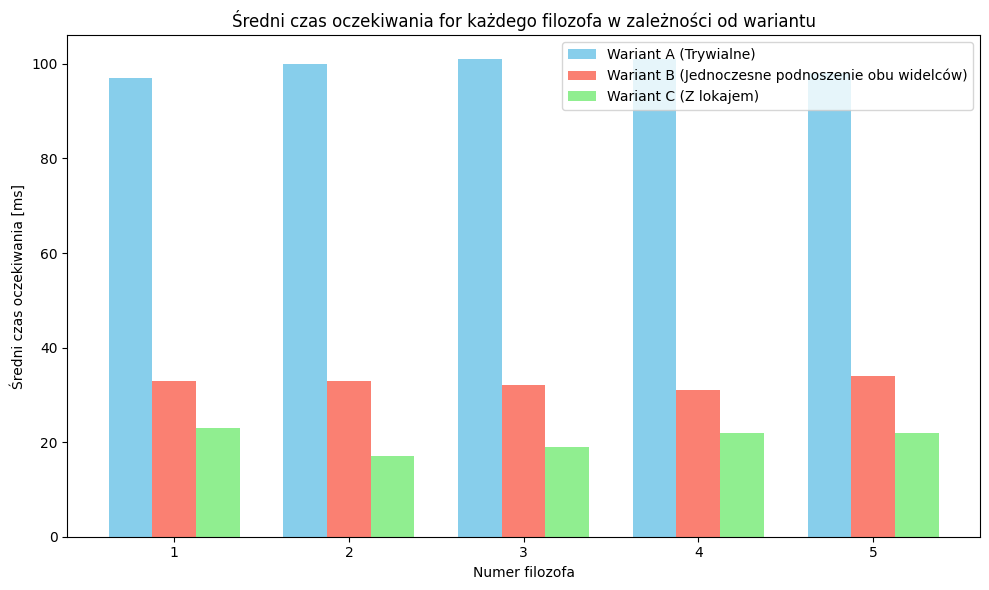
\includegraphics[width=12cm]{./graph.png}
\end{center}
\subsection*{Wnioski}
\label{sec:org70c755e}
We wszystkich rozwiązaniach średni czas oczekiwania był podobny dla każdego z filozofów.
Wynika to z faktu, że wartości przekazywane do funkcji \texttt{sleep} są stałę, co oznacza że
każdy z filozofów pracuje w podobnym tempie i podobnie
często próbuje podnieść widelce.
Rozwiązanie trywialne jest nie tylko najmniej wydajne, ale również oczywiście błędne.
Najszybszym rozwiązaniem okazało się rozwiązanie z lokajem, co jest zgodne z oczekiwaniami.
\section*{Bibliografia}
\label{sec:org1efc06e}
\begin{itemize}
\item \href{https://pl.wikipedia.org/wiki/Problem\_ucztuj\%C4\%85cych\_filozof\%C3\%B3w}{Problem ucztujących filozofów}
\item \url{https://wazniak.mimuw.edu.pl/index.php?title=Programowanie\_wsp\%C3\%B3\%C5\%82bie\%C5\%BCne\_i\_rozproszone/PWR\_Wyk\%C5\%82ad\_9}
\end{itemize}
\end{document}
